\begin{figure}[!tbhp]
  \centering
  \begin{subfigure}[b]{0.24\columnwidth}
    \centering
    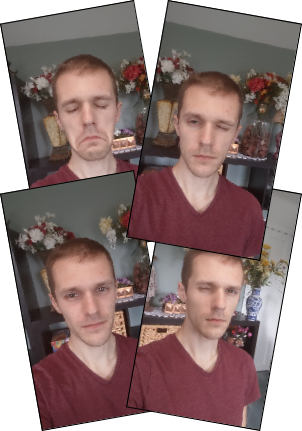
\includegraphics[width=\linewidth]{fig/\conerfdirname/assets/input images.png}
    \caption{}
  \end{subfigure}
  \hfill
  \begin{subfigure}[b]{0.12\columnwidth}
    \centering
    \includegraphics[width=\linewidth]{fig/\conerfdirname/assets/annotation.pdf}
    \caption{}
  \end{subfigure}
  \hfill
  \begin{subfigure}[b]{0.56\columnwidth}
    \centering
    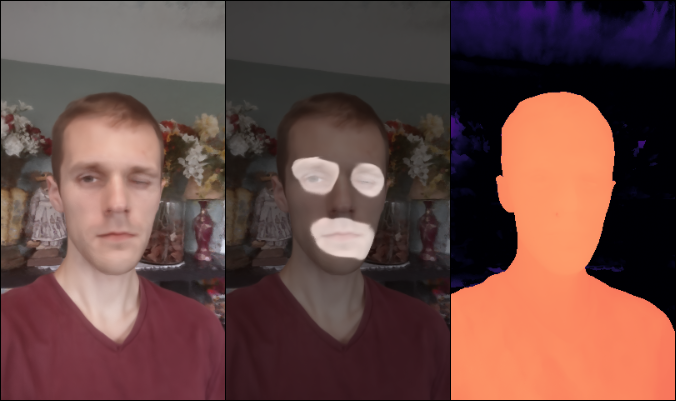
\includegraphics[width=\linewidth]{fig/\conerfdirname/assets/target.png}
    \caption{}
  \end{subfigure}
  \caption{
    Training a single attributed NeRF is structured as follows.
    We firstly capture set of images with a handheld smartphone camera (a).
    Then we provide annotations using an open source software (b).
    Finally, we train train model to reconstruct RGB colors and masks using
    volumetric rendering (c) \cite{mildenhall2020nerf}.
  }
  \label{fig:conerf-capture-pipeline}
\end{figure}